\documentclass[a4paper,11pt]{article}

\setlength{\parindent}{0pt}

% Various packages
\usepackage{graphicx}
\usepackage{a4wide}
\usepackage{url}
\usepackage[left=2cm,top=2cm,bottom=1.5cm,right=2cm]{geometry}
\usepackage{amsmath}
\usepackage{amssymb}
\usepackage{amsthm}
\usepackage{amsfonts}
\usepackage{wrapfig}
\usepackage{fixme}
\usepackage{color}
\usepackage{pstricks}
\usepackage{pdfpages}
\usepackage[utf8]{inputenc}
\usepackage{enumitem}
\usepackage{tasks}
\usepackage{float}
\usepackage{dutchcal}

%\usepackage{minted}

\usepackage{listings}
\usepackage{lstautogobble}
\usepackage{semantic}

% Various custom commands
\newcommand{\argmin}{hrm{argmin}}
\newcommand{\R}{\mathbb{R}}
\newcommand{\E}{\mathbb{E}}
\newcommand{\mean}{\mathbb{E}}
\newcommand{\V}{\mathbb{V}}
\newcommand{\prob}{\mathbb{P}}
\newcommand{\var}{\mathrm{var}}
\newcommand{\iid}{\overset{\text{iid}}{\sim}}

\newcommand{\w}{{\mathbf w}}
\newcommand{\x}{{\mathbf x}}
\newcommand{\y}{{\mathbf y}}
\newcommand{\X}{{\mathbf X}}
\renewcommand{\P}[1]{\mathbb P\lrc{#1}}
\DeclareMathAlphabet{\mathpzc}{OT1}{pzc}{m}{it}

\newcommand{\lr}[1]{\left (#1\right)}
\newcommand{\lrc}[1]{{\left \{#1\right\}}}
\newcommand{\lra}[1]{\left |#1\right|}
\newcommand{\lrs}[1]{\left [#1\right]}


\lstset{basicstyle=\ttfamily,
  mathescape=true,
  escapeinside=||,
  autogobble}

\makeatletter
\newcommand*\bigcdot{\mathpalette\bigcdot@{.5}}
\newcommand*\bigcdot@[2]{\mathbin{\vcenter{\hbox{\scalebox{#2}{$\m@th#1\bullet$}}}}}
\makeatother
\usepackage{geometry}
\geometry{
  top=1.3in,    
  inner=1.4in,
  outer=1.4in,
  bottom=1.3in,
  headheight=3ex,  
  headsep=3ex,     
}
\usepackage{fancyhdr}
\pagestyle{fancyplain}
\pagestyle{fancy}
\fancyhf{}
\fancyhead[LE,RO]{Matilde Broløs}
\fancyhead[RE,LO]{PLD - Assignment 1}
\fancyfoot[CE,CO]{}
\fancyfoot[LE,RO]{\thepage}
\renewcommand{\plainheadrulewidth}{0.4pt}

%\usepackage{tikz}


% Making itemized lists that save space
\newenvironment{packed_itemize}{
\begin{itemize}
  \setlength{\itemsep}{1pt}
  \setlength{\parskip}{0pt}
  \setlength{\parsep}{0pt}
}{\end{itemize}}


\title{PLD Assignment 1}
\author{Matilde Broløs (jtw868)}
\date{\today}

\begin{document}

\maketitle

\section*{A 1.1}

\subsection*{a)}
The contents of the file \textit{assignment1.le} are shown below.

First the \texttt{reverse} function.
\begin{verbatim}
\ Assignment 1
(load listfunctions)

\ A function 'reverse' that reverses a list
(define reverse (lambda ((a . d)) (append (reverse d) (list a)) (a) a))
\end{verbatim}
The function is recursively appending its first element to the back of the list that is generated by using the reverse function on the tail of the list.

To implement the second function, \texttt{sort}, I have implemented a number of helper functions, as seen below.
\begin{verbatim}
\ Helper function: append two lists (even if both lists are ())
(define append2
   (lambda (() bs) bs
           (bs ()) bs
           (() ()) ()
           ((a . as) bs) (cons a (append2 as bs))
           (bs (a . as)) (append (list bs a) as)
           (as bs) (list as bs)))

\ Helper function: Find all elements smaller than p
(define allSmallerThan (lambda ((a . d) p) (append2 (< a p) (allSmallerThan d p))
                               (() p) ()
                               (a p) (< a p)))

\ Helper function: Find all elements greater than p
(define allGreaterThan (lambda ((a . d) p) (append2 (> a p) (allGreaterThan d p))
                               (() p) ()
                               (a p) (> a p)))

\ A function 'sort' that sorts a list
(define sort (lambda ((a . d)) (append (append (sort (allSmallerThan d a)) 
                                       (list a)) (sort (allGreaterThan d a)))
                     (()) ()
                     a a))

\end{verbatim}
The idea behind the code is to choose a pivot element, which is simply the first element of the given list, and then divide the rest of the list in to two different lists - one where all elements are smaller than the pivot element, and on where all elements are larger or equal. Now the sort function is used recursively on both lists. The function returns a list consisting of first the list with smaller elements (sorted), then the pivot element, and then the list with larger or equal elements (sorted).

\subsection*{b)}
Here are some examples of running \texttt{reverse}.
\begin{figure}[h]
    \centering
    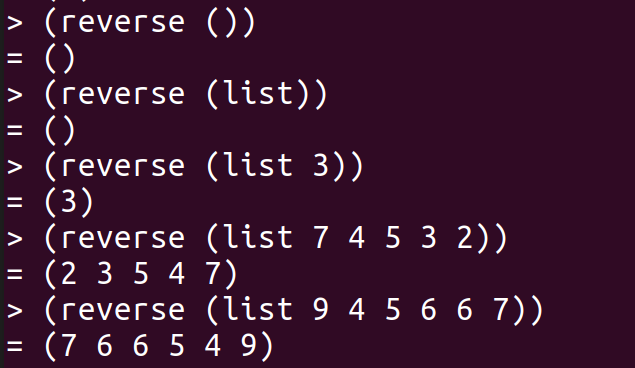
\includegraphics[width=0.5\textwidth]{rev.png}
    \caption{The reverse function}
\end{figure}

Here are some examples of running \texttt{sort}.
\begin{figure}[h]
    \centering
    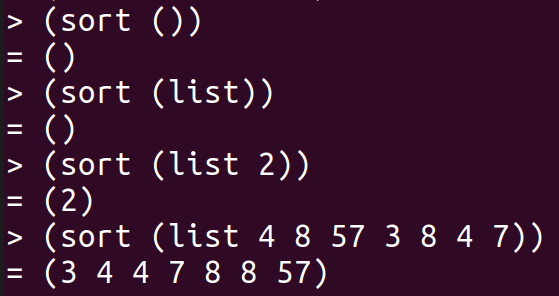
\includegraphics[width=0.5\textwidth]{sort.png}
    \caption{The sort function}
\end{figure}


\subsection*{c)}
I think the part of the syntax that was the most difficult for me to understand was the \textit{cons} operater, and the way the pattern matching work. I think the idea is pretty straight forward, but i spent quite a lot of time just trying out all of the operators to figure out exactly how they worked and what they returned.

\section*{A 1.2}

\subsection*{a)}
Below the programs and the machine is represented as diagrams (H is short for Haskell).
\begin{center}
  \begin{picture}(230,100)(-90,-20)
    \put(-30,0){\compiler{C,ARM,ARM}}
    \put(-130,0){\compiler{H,H,C}}
    \put(80,0){\interpreter{H,C}}
    \put(180,0){\machine{ARM}}
  \end{picture}
\end{center}

\subsection*{b)}
First we want to convert the interpreter of Haskell in C to an interpreter of Haskell in ARM:
\begin{center}
  \begin{picture}(230,100)(-90,-20)
    \put(0,0){\compiler{\interpreter{H,C},\machine{ARM},\interpreter{H,ARM}}}
  \end{picture}
\end{center}
So now we have the interpreter in ARM, and so we want to interpret the compiler from Haskell to C written in Haskell so we get a compiler from Haskell to C written in ARM.
\begin{center}
  \begin{picture}(230,150)(-20,-90)
    \put(0,0){\compiler{H,\compiler{H,\interpreter{H,\machine{ARM}},\compiler{H,\compiler{C,\machine{ARM},\compiler{H,ARM,C}},C}},C}}
%    \put(0,0){\compiler{\compiler{H,H,C},\interpreter{H,\machine{ARM}},\compiler{\compiler{H,C,C},\machine{ARM},\compiler{H,ARM,C}}}}
  \end{picture}
\end{center}
After running this, we have a compiler from Haskell to C written in ARM:
\begin{center}
  \begin{picture}(230,100)(-90,-20)
    \put(0,0){\compiler{H,ARM,C}}
  \end{picture}
\end{center}

\subsection*{c)}
Now we want to convert a program \textit{p} written in Haskell to a program written in ARM, using our new compiler. This can be done on our ARM machine as shown below.
\begin{center}
  \begin{picture}(230,100)(-20, -20)
    \program{p,\compiler{H,\machine{ARM},\program{p,\compiler{C,\machine{ARM},\program{p,ARM}}}}}
  \end{picture}
\end{center}

\section*{A 1.3}
I assume that a bit representation has the least significant bit to the right, and the most significant bit to the left, and I therefore count from right to left when iterating through the bits.

\subsection*{a)}
To make a function that can determine which type a bit representation \textit{rep} has, we need to extract different bits to see their value. We know the following:
\begin{enumerate}
	\item A \textit{number} is the only representation that has $1$ as the $2$'nd bit.
	\item A \textit{NIL} value has only $0$'s.
	\item A \textit{symbol} has a $1$ as the $34$'th bit, and all bits after that bit is $0$.
\end{enumerate}
Now to make the function \texttt{kind} we need to check these $3$ conditions. If neither of them are the case, the representation must be a \textit{pair}. Below a suggestion for pseudocode is given. When using \textbf{AND} the operation is a \textit{bitwise} and, and when \textbf{/\textbackslash} is used it is a logical and. When writing the bit string I indicate that it is a binary number by the suffix $\_2$.
\begin{verbatim}
kind (rep):
  if (rep AND 3) == 2:
    return 1 ; A number
  else if rep == 0:
    return 0 ; NIL
  // Extract index i by bit shifting
  i = rep >> 33
  else if i == 1;
    return 2 ; A symbol
  else
    return 3 ; A pair 
\end{verbatim}

\subsection*{b)}
To make a function that determines if two representations are equal, lets start by looking at the different types. 
\begin{itemize}
	\item If two representations are both NIL, we can determine if they are the same by simply checking if they have the same value.
	\item If two representations are both numbers, we can again determine if they are equal by checking if their values are the same.
	\item If two representations are both symbols, we know that for them to be equal both $j$ indexes must be the same. The rest of the representation is predefined, so in this case we also simply have to check that the values of the bit representations are the same.
	\item Now, for a pair we know that two pairs can be equal, even if they dont point to the same indexes in the heap. Thus, we cannot just compare the values of the representations in this case. We need to extract the indexes from the representations, and then check whether the values at the given indexes in the heap are equal.
\end{itemize}
Thus, we have our cases for the function. Below a suggestion for the pseudocode is presented. When extracting the value at the x'th index from the heap is is represented as $heap(x)$.
\begin{verbatim}
equal (rep1, rep2):
  if kind(rep1) != kind(rep2):
    return FALSE
  else if kind(rep1) != 3:
    return (rep1 == rep2)
  else
    // Extract index i by bit shifting
    i1 = rep1 >> 33
    i2 = rep2 >> 33
    // Extract index j by AND'ing with bit value: 31x0 + 31x1 + 2x0 = 64 bits
    j1 = rep1 AND 0x1FFFFFFFC
    j2 = rep2 AND 0x1FFFFFFFC
    
    return (heap(i1) == heap(i2)) /\ (heap(j1) == heap(j2))
\end{verbatim}



\subsection*{c)}
What kind of fragmentation can mark-sweep cause? As I understand, the structure of the heap is that it is build up of a lot of chunks that are all $64$ bits. The values stored in the heap cannot excede $64$ bits, and at the same time we know that they all use exactly $64$ - thus, as I see it, there can be no kind of fragmentation, if we assume that we can keep track of what indexes in the heap are unused, as we will always need exactly $64$ bits for storing a value. Thus, the mark-sweep will not cause fragmentation, if we assume that the free indexes are kept track of.

\subsection*{d)}
The following is a suggestion as to how the \textit{mark-sweep-collection} could be modified to handle garbage collection in the symbol array. This assumes that all symbol values holds an index \textit{j} to the symbol array, and not the heap.

\begin{verbatim}
mark-and-sweep()
  set b to start of array
  WHILE b =< end-of-array DO
    IF b == NULL DO  
      go to next character in the array
    ELSE
      loop through all symbol pointers p
        IF p points to b DO
          go to next character in the array that is NULL
      set b = NULL 
\end{verbatim}

This code should loop through all indices in the symbol array: if the character is NULL, it goes to next character. If not, it loops through all symbols to check whether any of them points to this index. If the index is pointed to, we go to the next index that holds a NULL value. If no symbol points to the index, we set the value to NULL. After the mark-sweep all unused indices should have been set to NULL. When adding $n$ new characters, one must find $n + 2$ indices in a row, all holding the value NULL.


\end{document}
